% =============================================================================
% VALIDATION SECTION — drop into main.tex where RQ2 classification results appear
% Figures referenced: validation_comparison.png, usage_distribution.png
% Run analyse_validation.py to regenerate numbers if consensus.csv changes
% Status: single-rater preliminary (rater_MRG as consensus; rater_KQ pending)
% =============================================================================

\subsection{Manual Validation of LLM Usage Classification}
\label{sec:usage-validation}

The usage-type labels assigned by the LLM pipeline (Section~\ref{sec:classification-method})
were validated against independent human judgement on a stratified random sample of
repositories to assess the precision of each label.

\subsubsection*{Sampling design}
A stratified sample of 40 repositories was drawn from the 1{,}677 usage repositories,
with 10 repositories selected uniformly at random from each of the four LLM-assigned
label strata (\textit{actual\_usage}, \textit{framework\_library},
\textit{research\_artefact}, \textit{other\_usage}), using a fixed random seed for
reproducibility.
Each sampled repository was manually reviewed by visiting its GitHub page and reading
its README, code, and issue history; the rater recorded: binary labels for each
usage type (which may overlap), an \textit{other\_usage} sub-type where applicable,
a one-line evidence note, a confidence rating (high / medium / low), and time spent.

\subsubsection*{Precision of LLM labels}
Table~\ref{tab:llm-precision} reports LLM precision for each label: the proportion
of the 10 repositories that the LLM labelled as~$\ell$ which a human rater also
assigned label~$\ell$, with exact 95\% Clopper–Pearson confidence intervals.

\begin{table}[h]
\centering
\caption{LLM precision per usage label against manual consensus
         ($n = 10$ per label; 95\% Clopper–Pearson CI).
         \emph{Note:} wide intervals reflect the per-label sample size of 10;
         a two-rater consensus will narrow these bounds.}
\label{tab:llm-precision}
\begin{tabular}{lcccc}
\hline
\textbf{Label} & \textbf{LLM correct} & \textbf{Precision} & \textbf{95\% CI} \\
\hline
Actual usage         & 6 / 10 & 60\% & 26\%–88\% \\
Framework / library  & 3 / 10 & 30\% & 7\%–65\%  \\
Research artefact    & 6 / 10 & 60\% & 26\%–88\% \\
Other                & 7 / 10 & 70\% & 35\%–93\% \\
\hline
\end{tabular}
\end{table}

The \textit{framework\_library} label showed the lowest precision (30\%, CI 7–65\%).
Manual review found that the LLM in several cases applied this label to generic
libraries or tools that \emph{use} metamorphic testing to verify their own code
rather than providing MT infrastructure to downstream users.
This definitional boundary is acknowledged in the classification protocol
(Section~\ref{sec:classification-method}), and the overlap with \textit{actual\_usage}
means affected repositories are still correctly identified as MT-active.

\subsubsection*{LLM–human agreement across all sampled repositories}
As a secondary measure, Table~\ref{tab:llm-agreement} reports the overall agreement
rate and Cohen's~$\kappa$ between the LLM label and the human consensus
across all 40 sampled repositories for each label.

\begin{table}[h]
\centering
\caption{LLM–human label agreement on all 40 sampled repositories.
         $\kappa$ benchmarks: $<$0.40 fair; 0.41–0.60 moderate;
         0.61–0.80 substantial~\cite{landis1977}.}
\label{tab:llm-agreement}
\begin{tabular}{lccc}
\hline
\textbf{Label} & \textbf{\% Agreement} & \textbf{Cohen's $\kappa$} & \textbf{Interpretation} \\
\hline
Actual usage         & 75.0\% & 0.49 & Moderate \\
Framework / library  & 70.0\% & 0.32 & Fair     \\
Research artefact    & 72.5\% & 0.36 & Fair     \\
Other                & 75.0\% & 0.41 & Moderate \\
\hline
\end{tabular}
\end{table}

Figure~\ref{fig:validation} visualises both measures.
All four labels sit below the $\kappa = 0.61$ threshold for \emph{substantial}
agreement, with \textit{actual\_usage} and \textit{other\_usage} closest to that
threshold ($\kappa = 0.49$ and 0.41 respectively).
The lower values for \textit{framework\_library} and \textit{research\_artefact}
($\kappa = 0.32$–0.36) are consistent with the definitional ambiguity noted above
and with the inherently subjective distinction between a tool that applies MT and
one that constitutes an MT framework.

\begin{figure}[h]
\centering
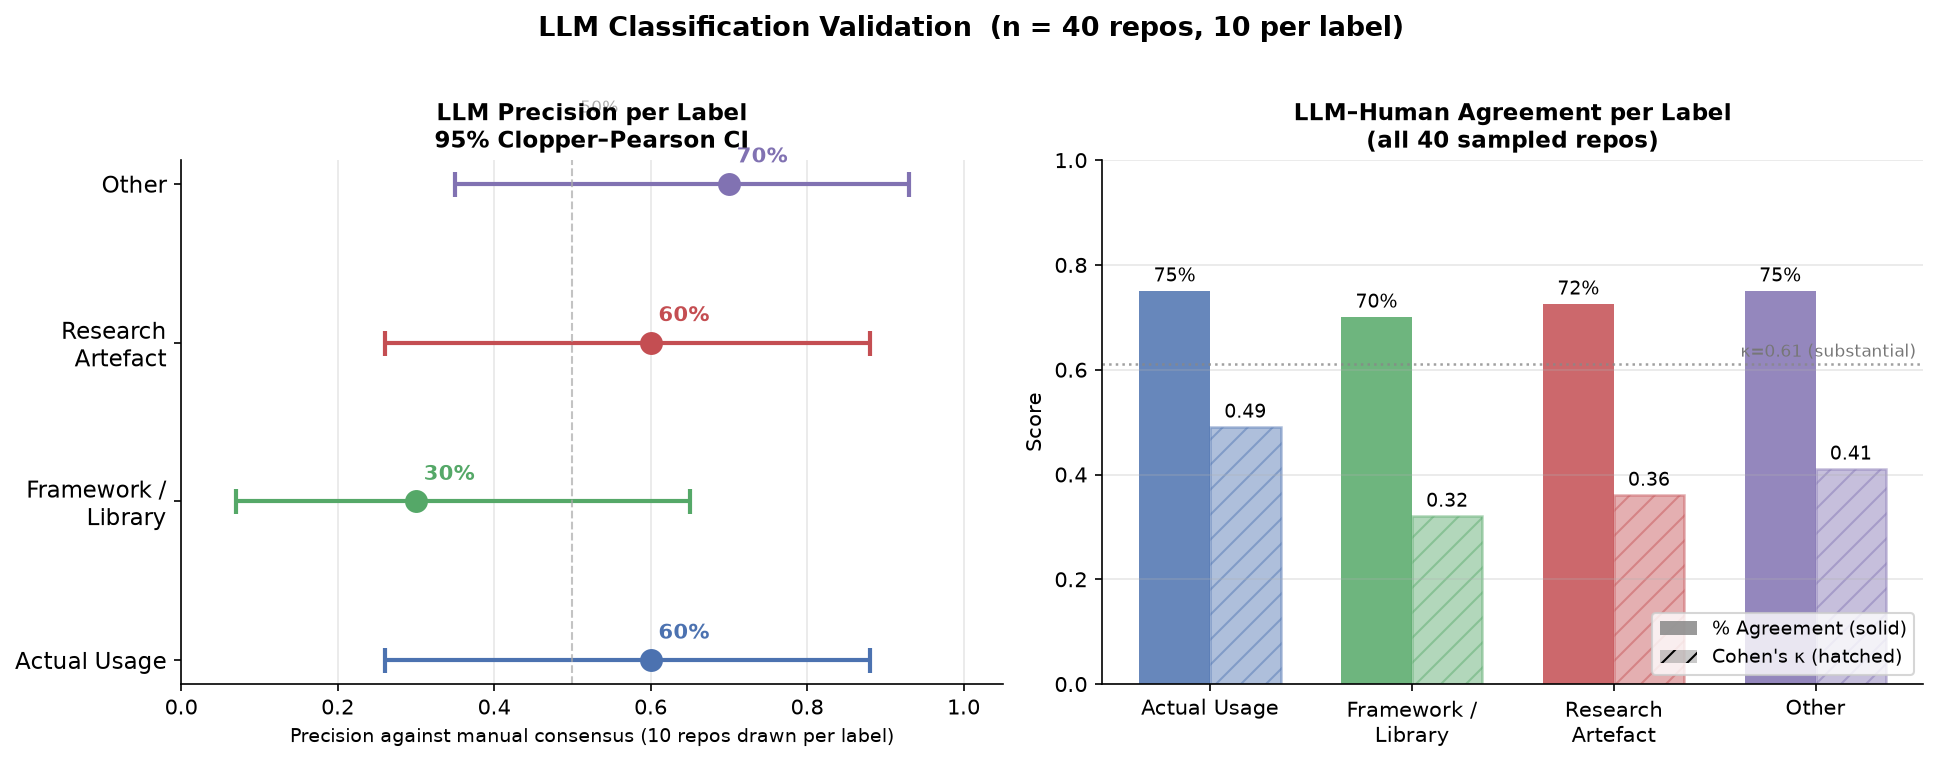
\includegraphics[width=\linewidth]{validation_comparison.png}
\caption{Left: LLM precision per usage label with 95\% Clopper–Pearson confidence
         intervals ($n = 10$ repos per label drawn from the stratified sample).
         Right: overall LLM–human agreement and Cohen's~$\kappa$ computed across
         all 40 sampled repositories.
         Dotted reference line at $\kappa = 0.61$ (substantial agreement).}
\label{fig:validation}
\end{figure}

\subsubsection*{False positives}
Seven of the 40 sampled repositories (17.5\%) were judged to contain no genuine
metamorphic testing at all: the keyword surface match originated from use of the
word \emph{metamorphic} in unrelated contexts (smart-contract metamorphism,
general-purpose code transformations, documentation references only, or AI agent
configuration files that mention the concept without implementation).
These false positives propagate into the reported usage counts; applying the
estimated 17.5\% false-positive rate to the full 1{,}677 usage repositories
implies an adjusted corpus of approximately $1{,}677 \times 0.825 \approx 1{,}383$
repositories with genuine MT involvement.

\subsubsection*{Limitations}
The results in this section are \emph{preliminary}: the consensus used here is
derived from a single rater (MRG); a second rater (KQ) is pending.
A two-rater consensus will provide inter-rater reliability statistics (Cohen's~$\kappa$
between raters) and may shift the precision estimates within the reported confidence
intervals.
The per-label sample of $n = 10$ yields wide confidence intervals; the Clopper–Pearson
bounds above should be treated as order-of-magnitude estimates rather than
precise characterisations of LLM performance.
